\section{Experimental Results}
\label{section:exp}
\subsection{Evaluation of Baseline Methods}
\label{section:exp:baseline}

Based on the experimental results evaluating validation scores against evaluation budgets, the following technical observations are made regarding the performance of the optimization algorithms:

\begin{figure}[htbp]
    \centering
    \begin{subfigure}[b]{0.48\textwidth}
        \centering
        % Insert the 20 budget image here
        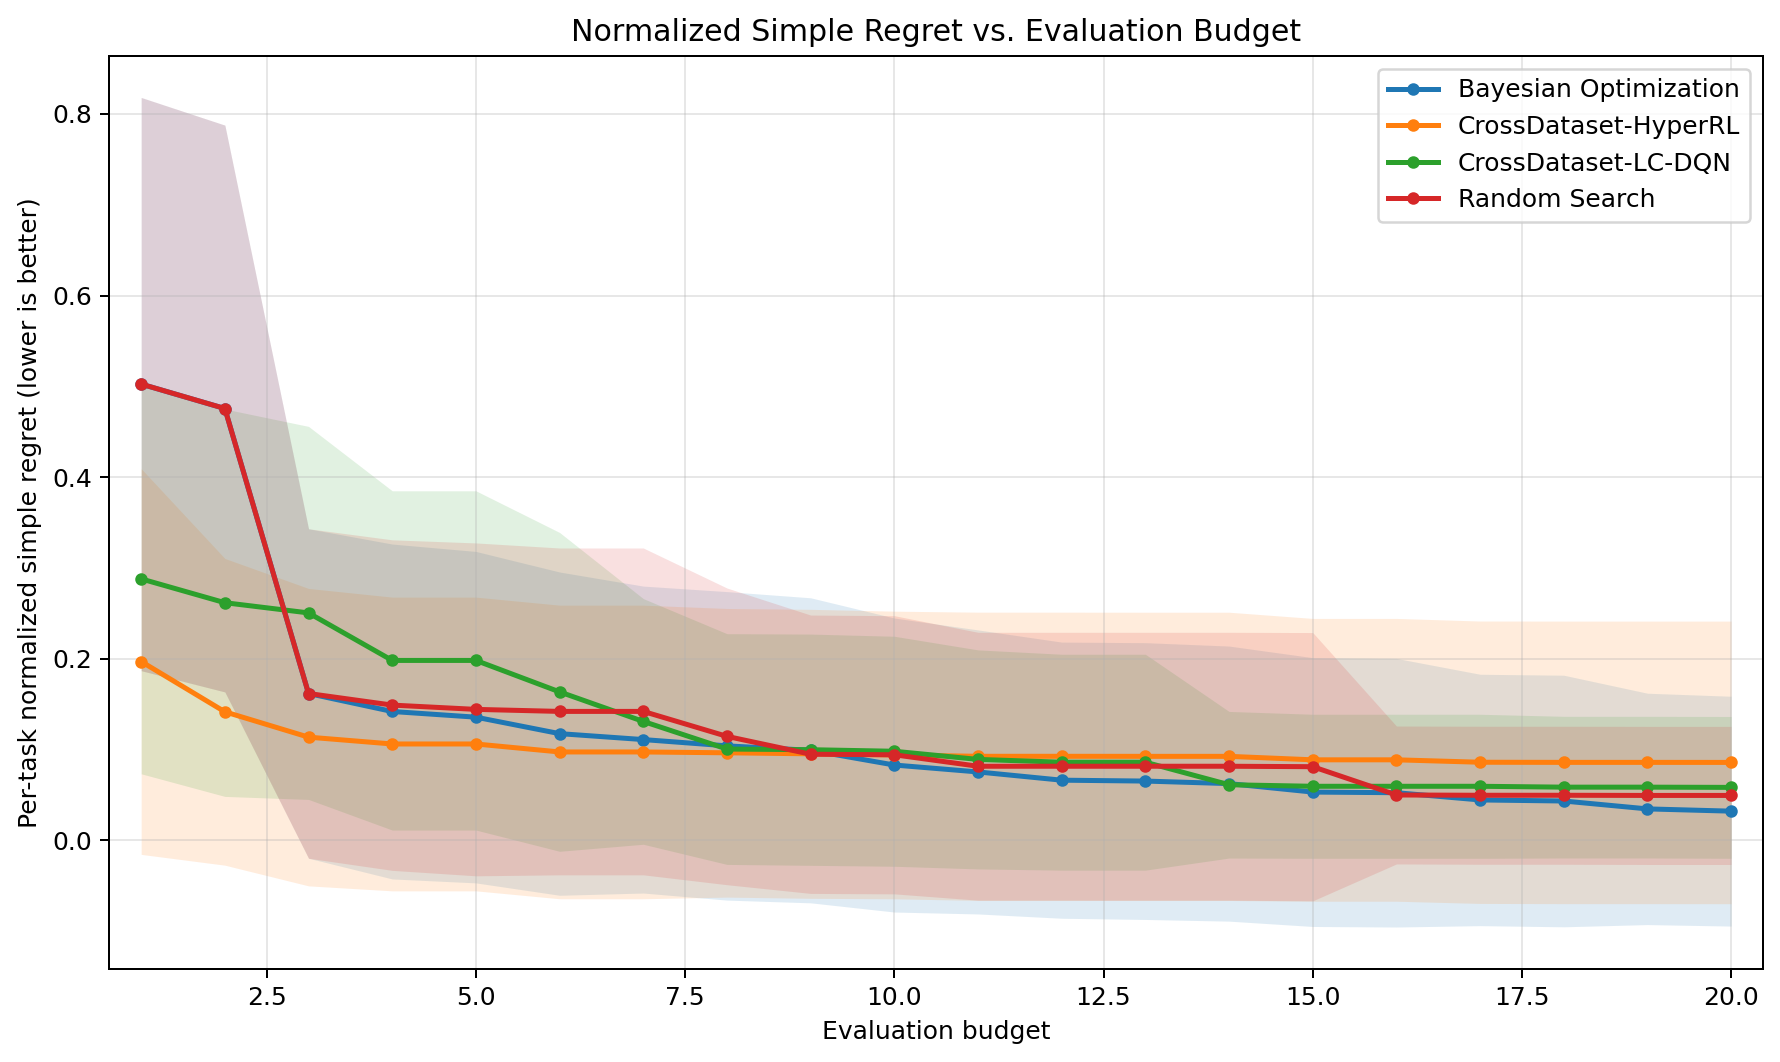
\includegraphics[width=\textwidth]{images/20_budget.png}
        \caption{Training Budget: 20}
        \label{fig:budget_20}
    \end{subfigure}
    \hfill
    \begin{subfigure}[b]{0.48\textwidth}
        \centering
        % Insert the 50 budget image here
        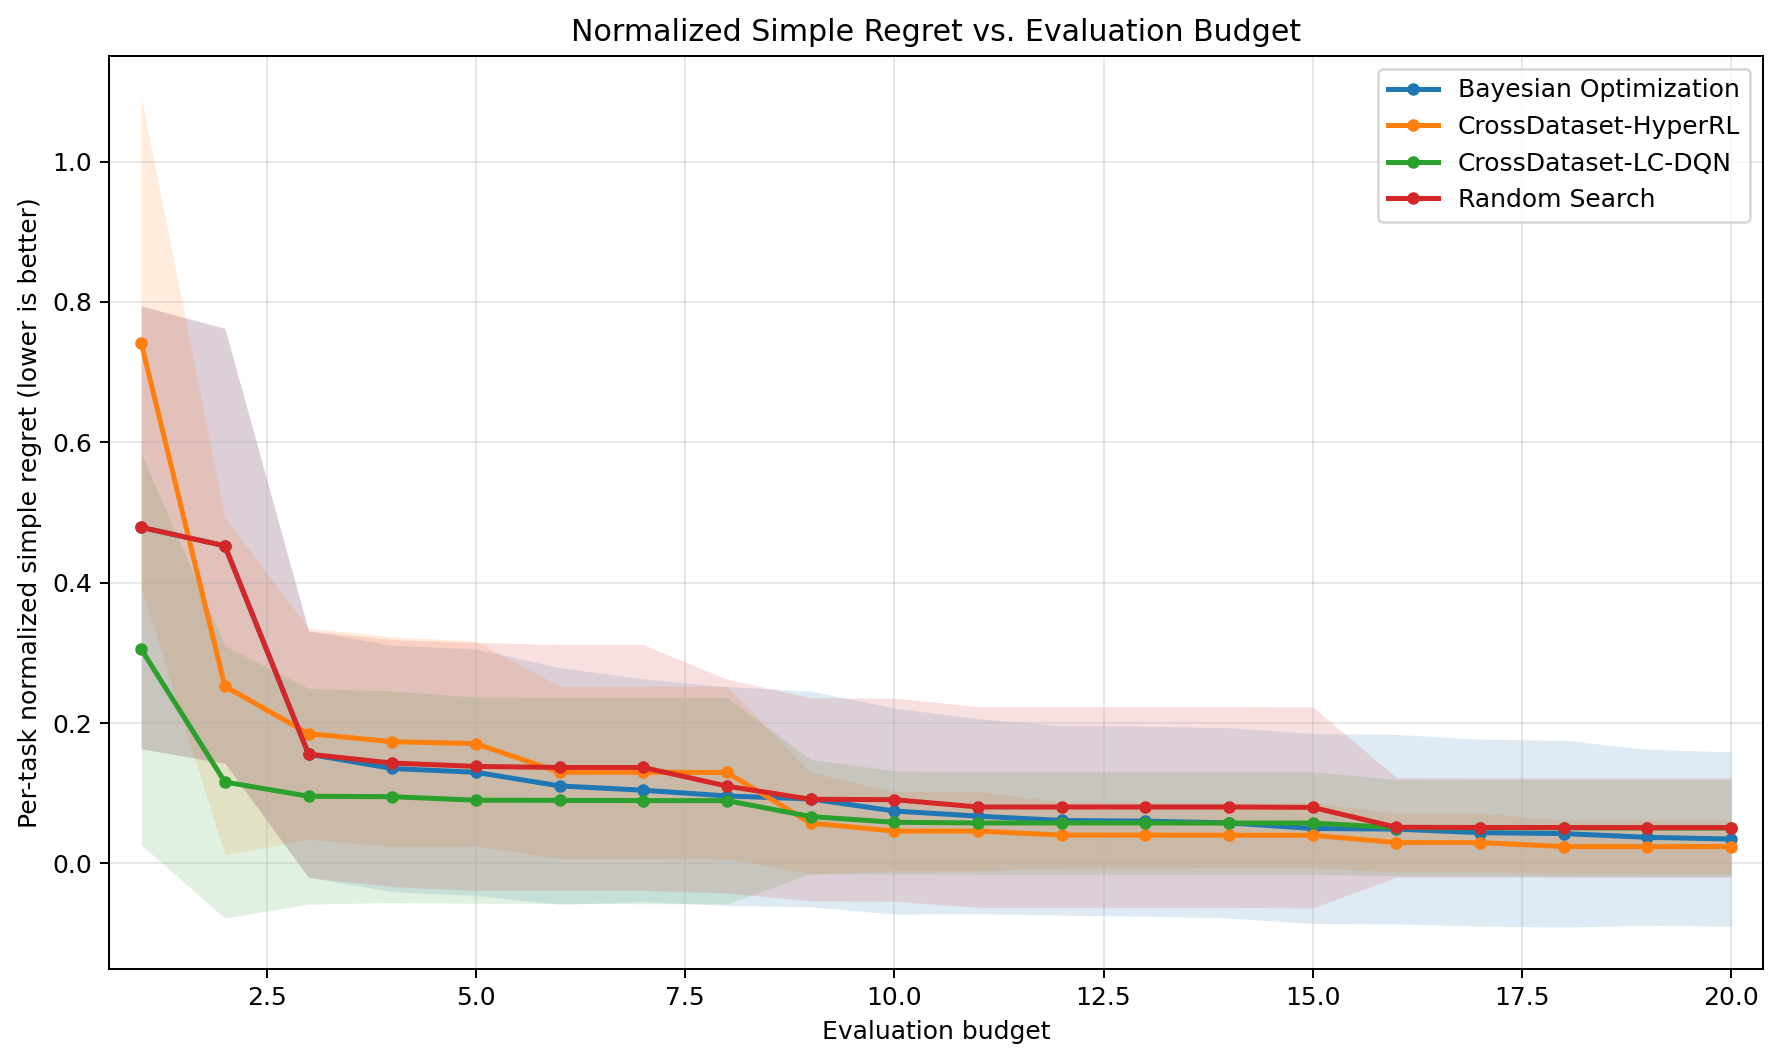
\includegraphics[width=\textwidth]{images/50_budget.png}
        \caption{Training Budget: 50}
        \label{fig:budget_50}
    \end{subfigure}
    
    % The empty line above and below the vspace is required to force a line break for the subfigures
    \vspace{0.5em}
    
    \begin{subfigure}[b]{0.48\textwidth}
        \centering
        % Insert the 100 budget image here
        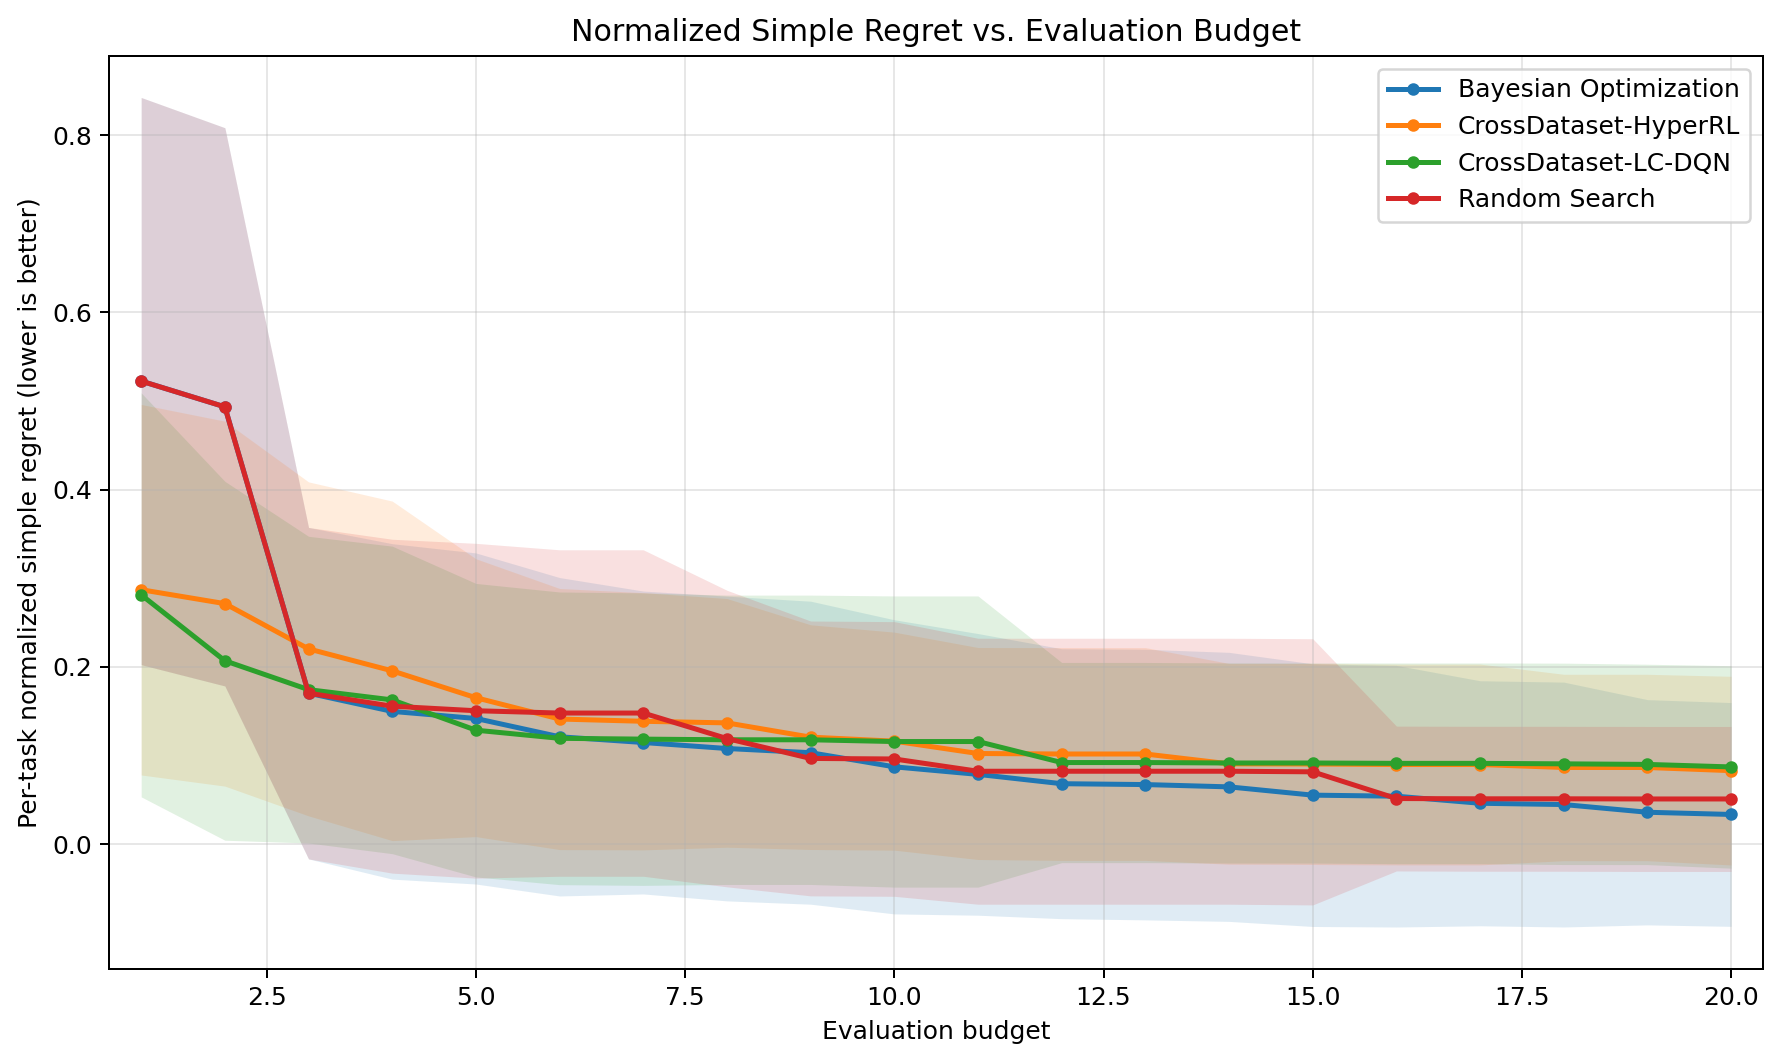
\includegraphics[width=\textwidth]{images/100_budget.png}
        \caption{Training Budget: 100}
        \label{fig:budget_100}
    \end{subfigure}
    \hfill
    \begin{subfigure}[b]{0.48\textwidth}
        \centering
        % Insert the 150 budget image here
        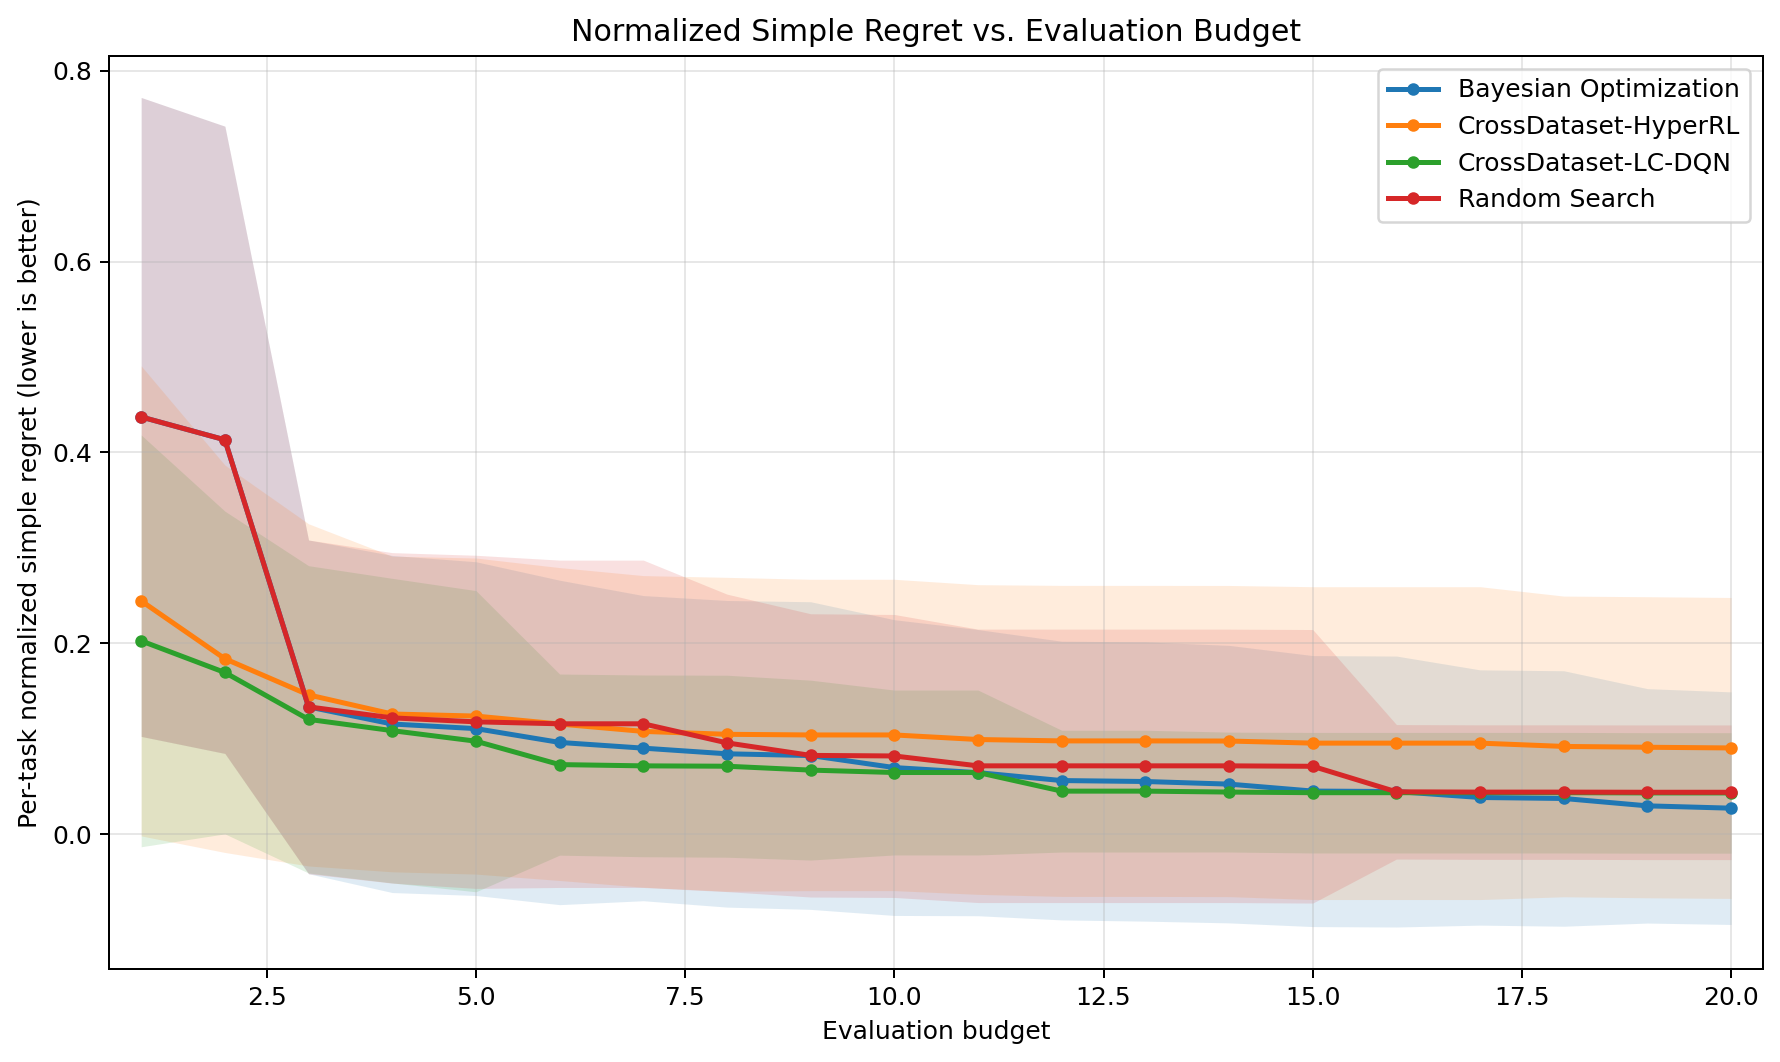
\includegraphics[width=\textwidth]{images/150_budget.png}
        \caption{Training Budget: 150}
        \label{fig:budget_150}
    \end{subfigure}
    \caption{Performance comparison of hyperparameter optimization methods across different training budget constraints. Lower validation scores indicate better performance.}
    \label{fig:hpo_results}
\end{figure}

\begin{itemize}
    \item \textbf{Initial Optimization Phase (Cold-Start):} At low evaluation budgets (e.g., trials 1 through 5), the \texttt{CrossDataset-HyperRL} and \texttt{CrossDataset-LC-DQN} methods yield lower validation scores compared to Bayesian Optimization and Random Search. This indicates a higher search efficiency and a more effective initialization during the early phase of the optimization process.
    \item \textbf{Meta-Learning and Knowledge Transfer:} This early-stage performance difference correlates with the underlying initialization mechanisms. \texttt{CrossDataset-HyperRL} utilizes metadata to transfer learned hyperparameter distributions from prior datasets to the current validation dataset. Conversely, standard Bayesian Optimization initiates the search process on each new dataset without prior external data, requiring more exploratory trials to model the objective function from scratch.
    \item \textbf{Asymptotic Convergence:} As the evaluation budget increases (beyond 15 to 20 trials), the validation scores of all evaluated methods converge to a similar numerical range. The data shows that given a sufficient evaluation budget, the surrogate model constructed by Bayesian Optimization achieves an equivalent performance level to the transferred policies of the meta-learning approaches.
\end{itemize}

